\section{Implementación de los resultados de los MoP de apuntamiento}

\label{ap:Z8}


Para mostrar el paso a paso de la cuantificación de los MoP de apuntamiento, se utilizará como ejemplo la simulación del SUCHAI-3 con los datos utilizados en el Capítulo 4, con los componentes físicos de nivel bajo en magnetorquer.

\underline{Jitter}

Para la cuantificación de este MoP de apuntamiento, en primera instancia se aplica el filtro pasa alto con una frecuencia tope de 10 Hz, mostrando solo las señales mayores a dicho valor. Con esto se observa la Figura \ref{fig:RPY_highpass} asentándose la señal siempre en el cero con el ruido de las vibraciones del sistema.

\begin{figure}[h!]
	\centering    
	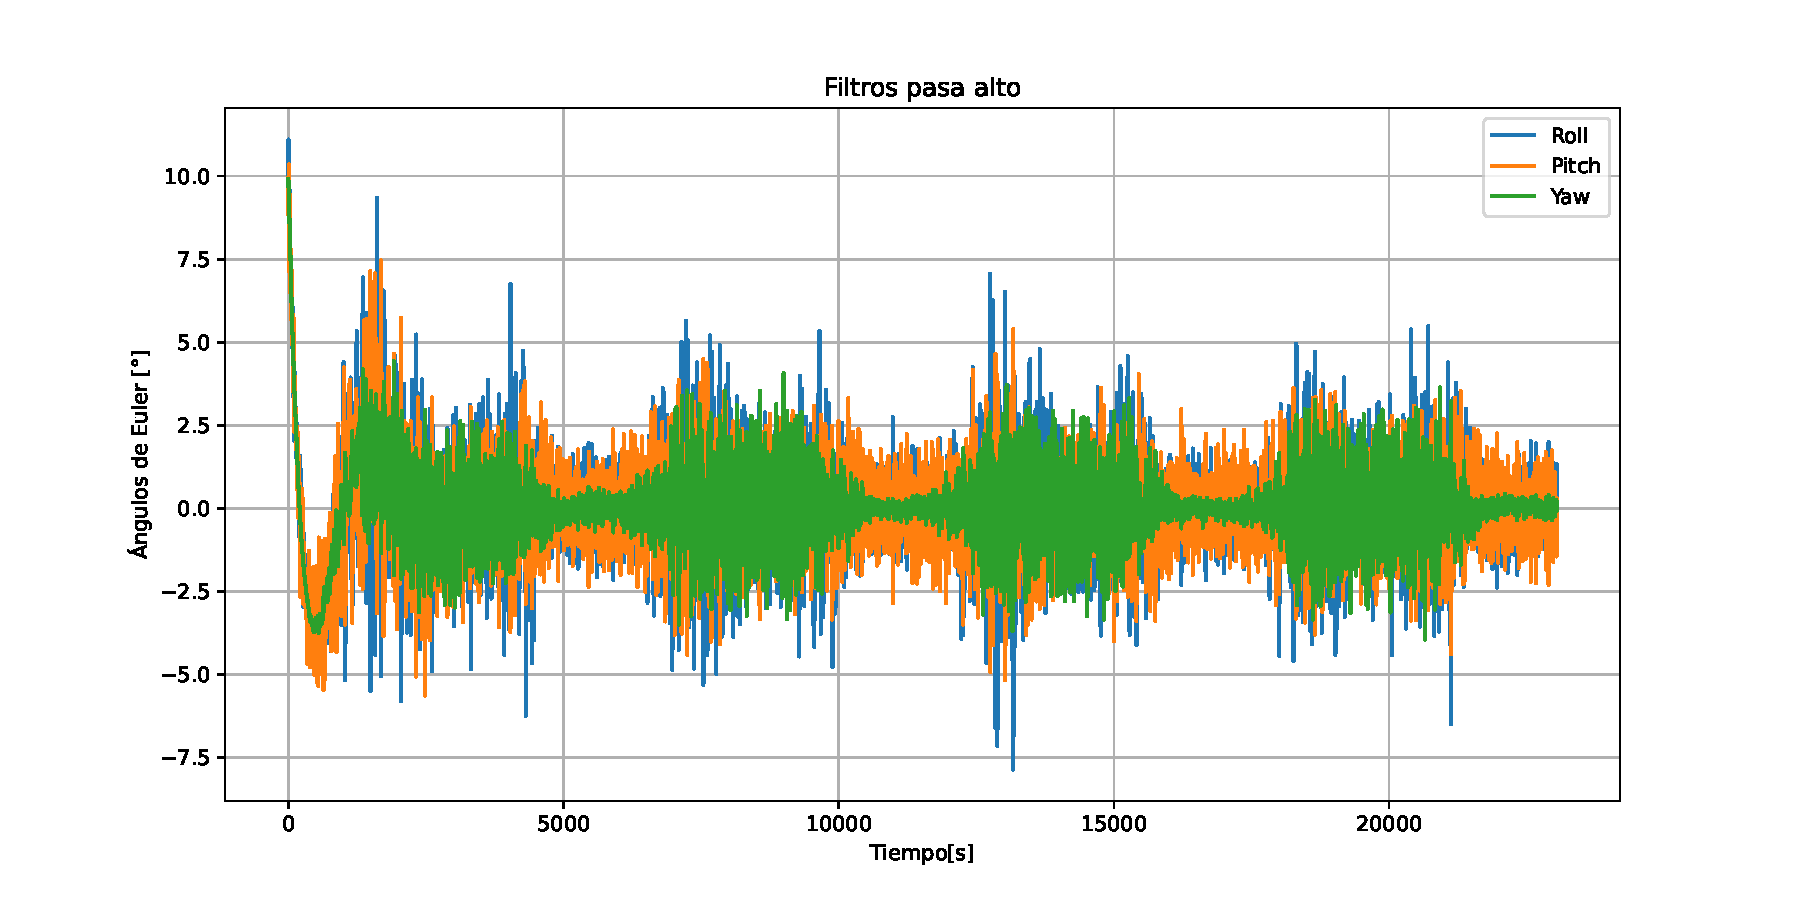
\includegraphics[width=0.9\textwidth]{RPY_highpass.pdf}
	\caption{Filtro pasa alto de 10 Hz en la respuesta al sistema de sensores y actuadores de nivel alto.}
	\label{fig:RPY_highpass}
\end{figure}	


Con esto, se obtienen las frecuencias y sus densidades espectro potencias aproximadas mediante la función welch de scipy.signal disponible en Python. Posteriormente, se selecciona todo el ancho de banda, para obtener el PSD que representa el jitter del sistema. Esto se observa en los ángulos de Euler en las Figura \ref{fig:psd_roll}, Figura \ref{fig:psd_pitch} y Figura \ref{fig:psd_yaw} para cada uno, presentado mayores valores a menores frecuencias. Se observa en el área pintada la integración dentro del ancho de banda realizada.

\begin{figure}[H]
	\centering    
	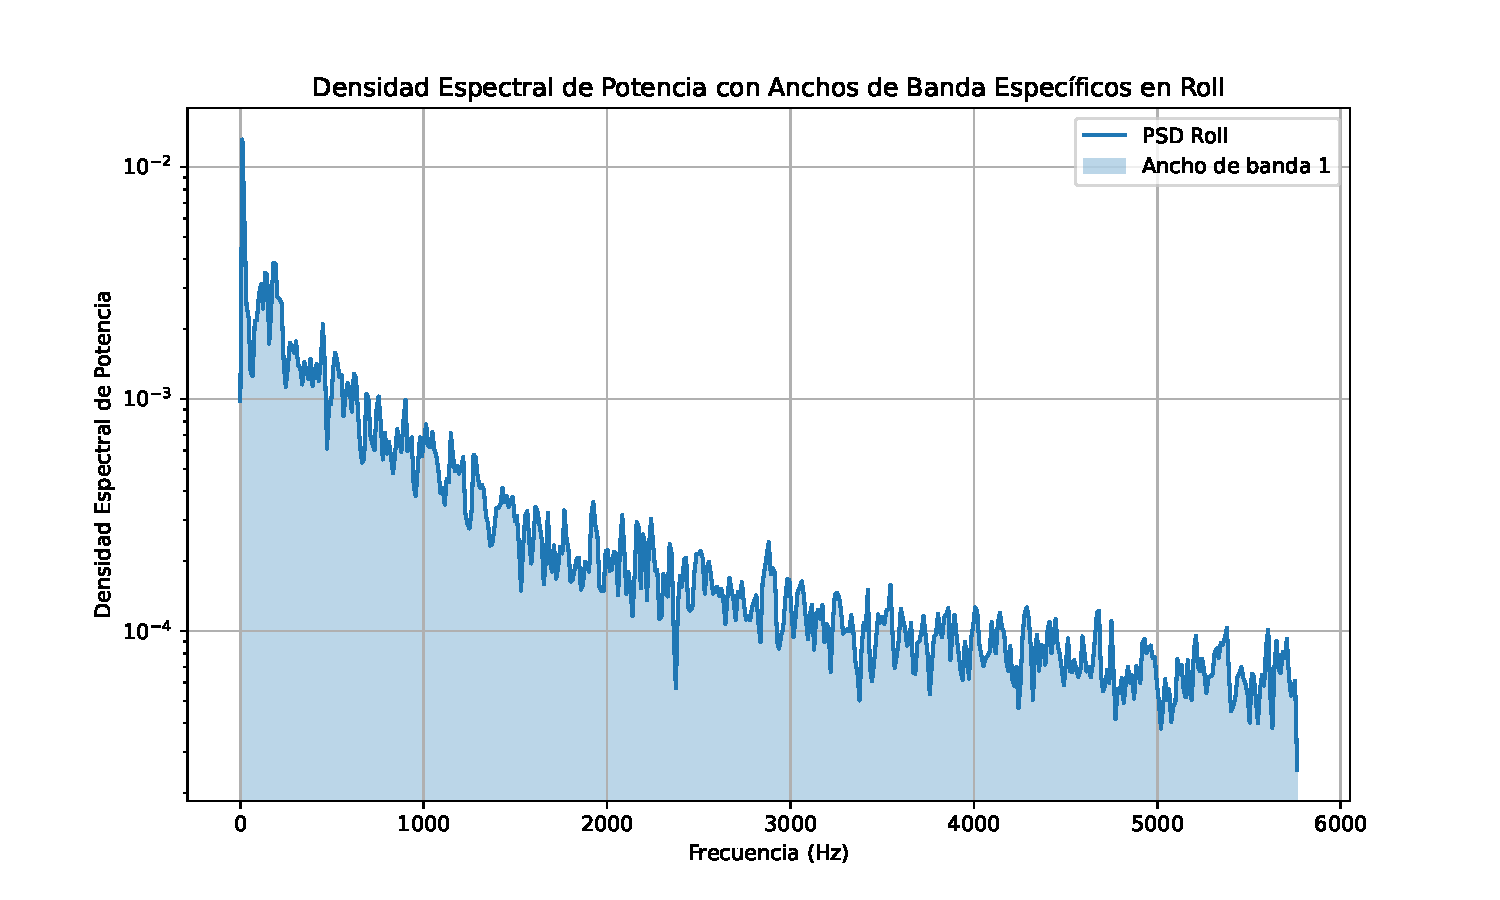
\includegraphics[width=0.8\textwidth]{psd_roll.pdf}
	\caption{Densidad espectro potencia en ancho de banda seleccionada para Roll.}
	\label{fig:psd_roll}
\end{figure}	

\begin{figure}[H]
	\centering    
	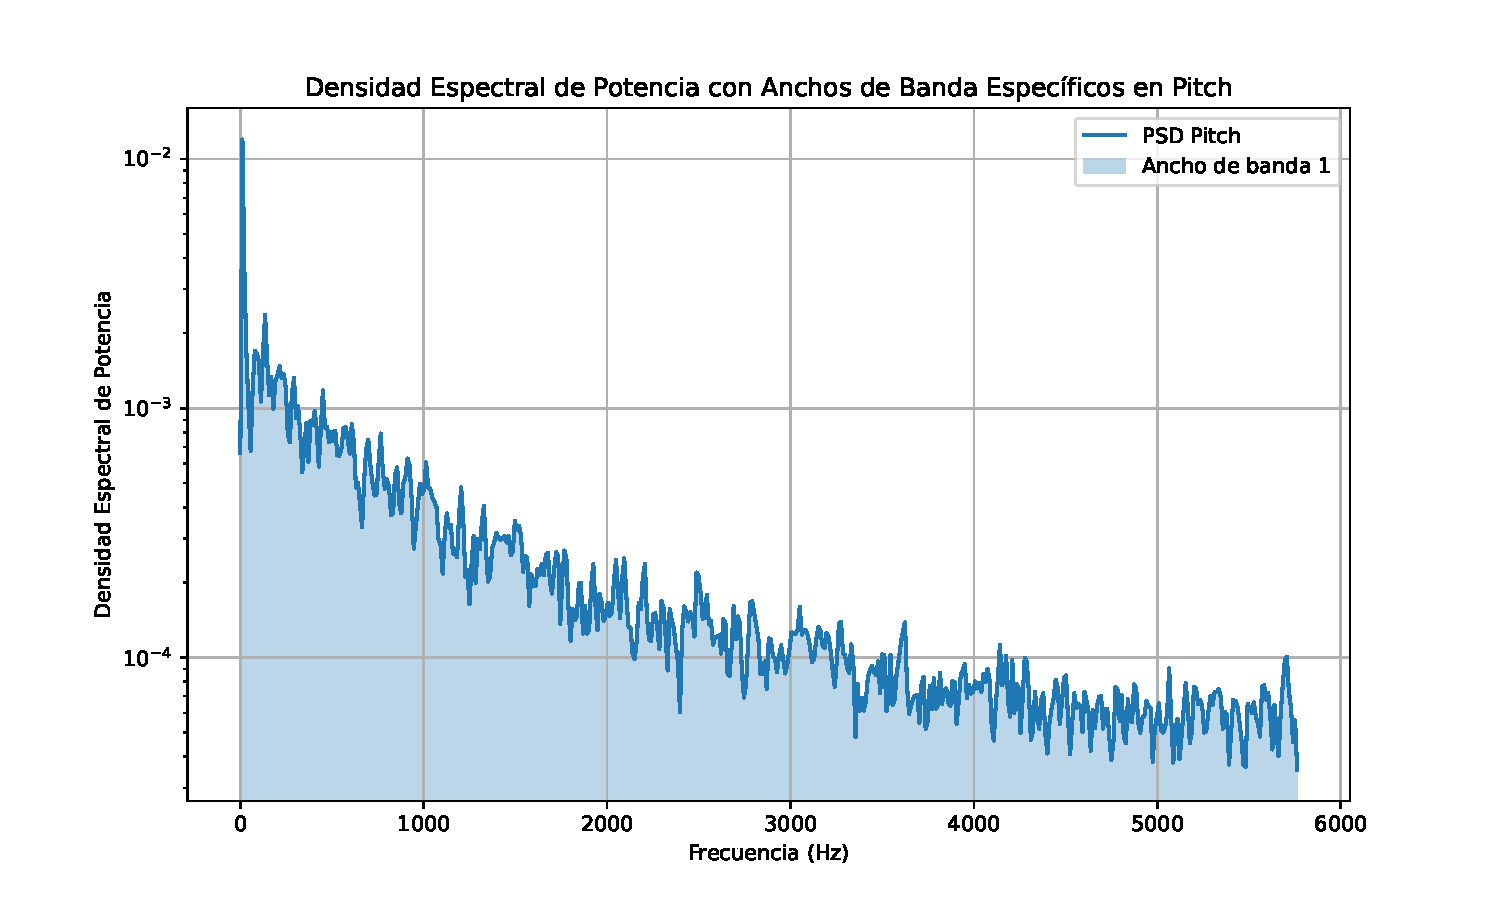
\includegraphics[width=0.8\textwidth]{psd_pitch.pdf}
	\caption{Densidad espectro potencia en ancho de banda seleccionada para Pitch.}
	\label{fig:psd_pitch}
\end{figure}	

\begin{figure}[H]
	\centering    
	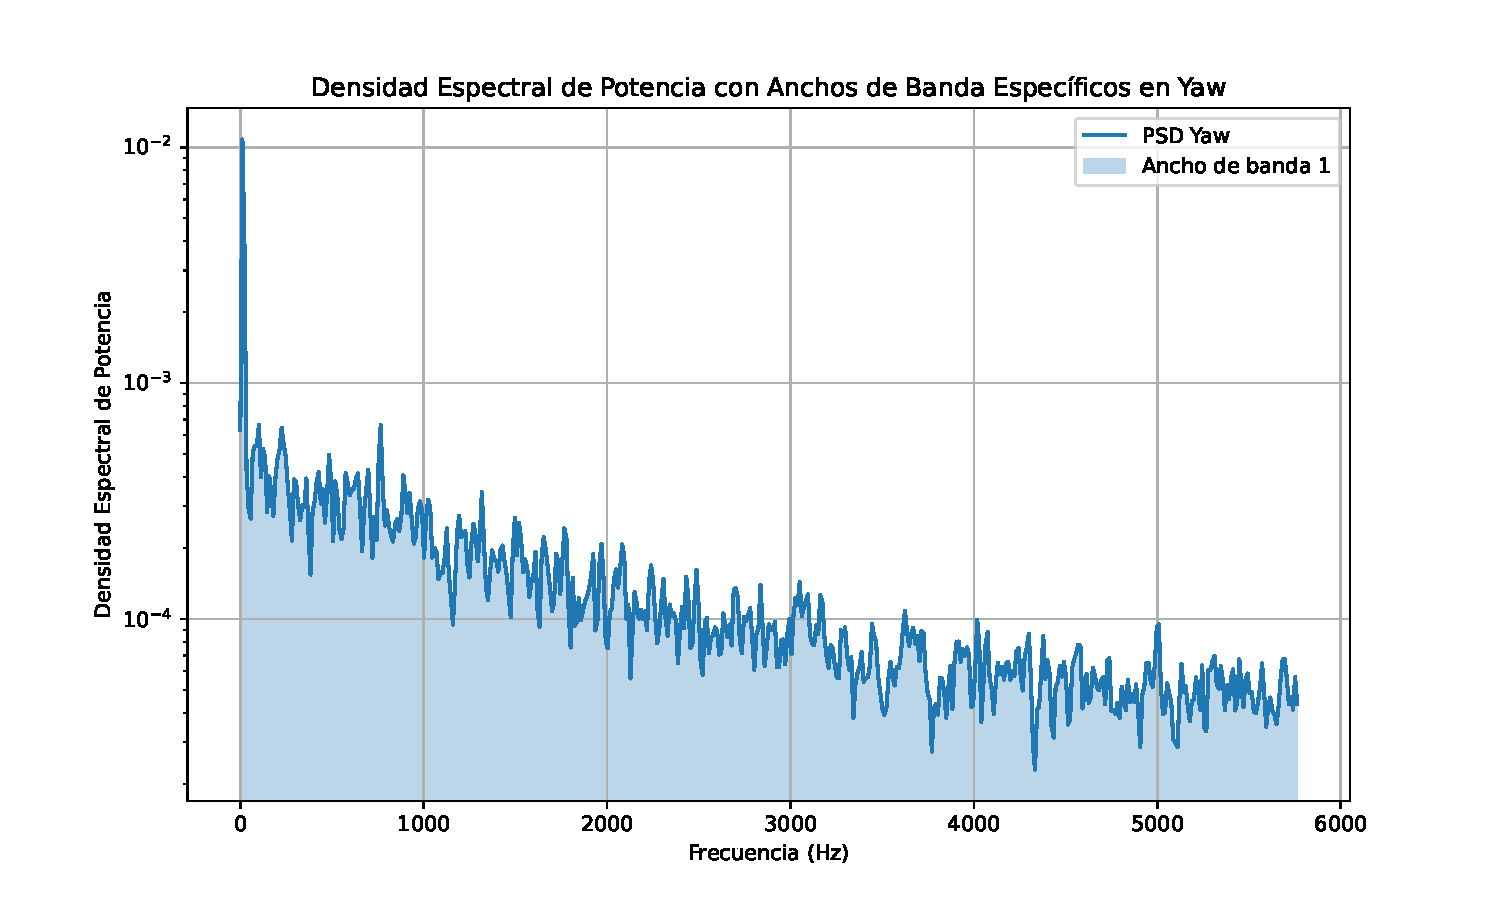
\includegraphics[width=0.8\textwidth]{psd_yaw.pdf}
	\caption{Densidad espectro potencia en ancho de banda seleccionada para Yaw.}
	\label{fig:psd_yaw}
\end{figure}	


\underline{Agilidad}

Por otro lado, para la cuantificación de la agilidad, se utilizan los valores de los angulos de Euler reales obtenidos por el modelo. Esto se hace con el objetivo de conocer lo más preciso posible el tiempo de asentamiento con una banda cercana al objetivo (entre -2.5 y 2.5 grados de los angulos de Euler) sin las perturbaciones causadas por el ruido de los sensores.

En las Figura \ref{fig:time_roll}, Figura \ref{fig:time_pitch} y Figura \ref{fig:time_yaw} se muestran los ángulos de Euler Roll, Pitch y Yaw reales, en conjunto con una gráfica acercada en la zona de asentamiento, mostrando además los limites superior e inferior dadas por la banda de asentamiento. Una vez que la orientación del satélite está presente dentro de la banda de asentamiento, el tiempo inicial para el ingreso sin retirarse es el tiempo de asentamiento con el cual se cuantifica la agilidad

\begin{figure}[H]
	\centering    
	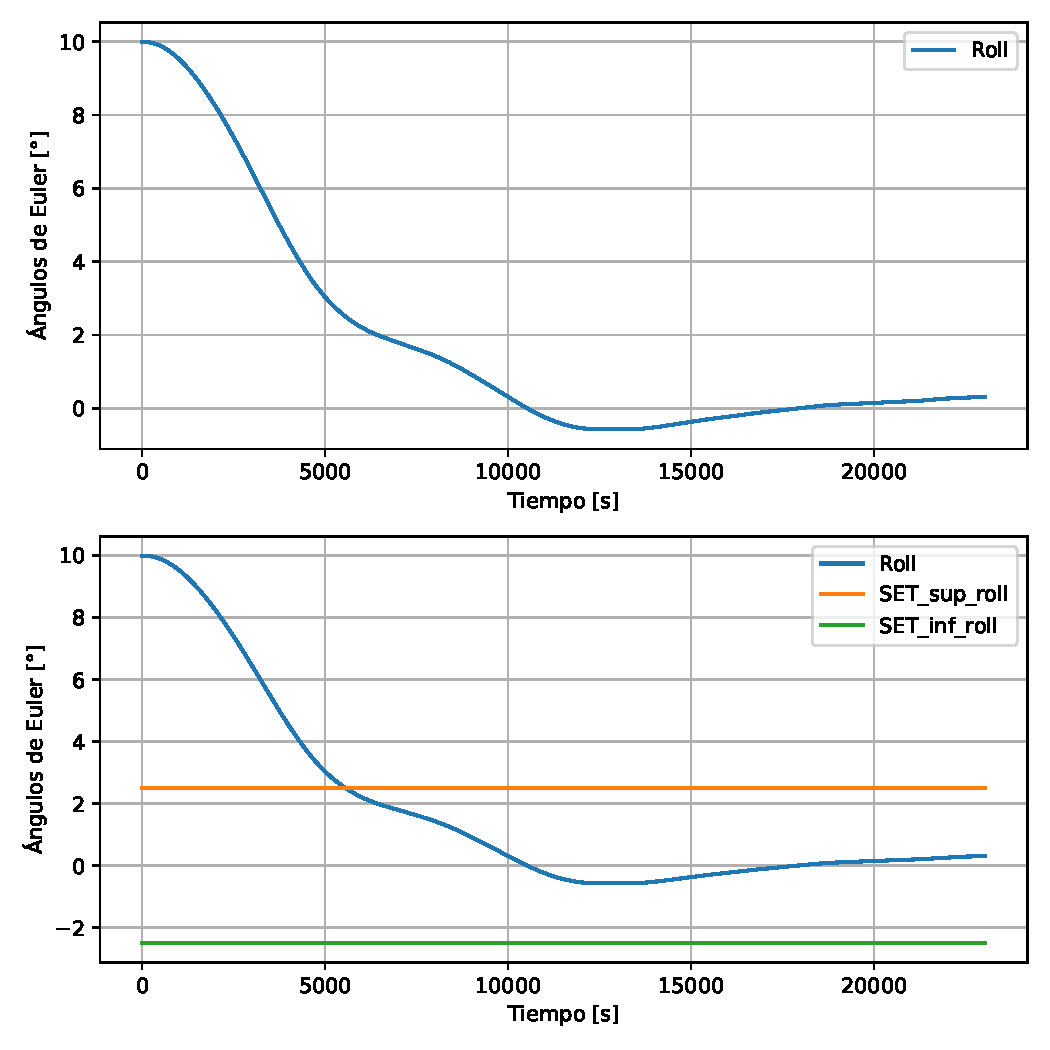
\includegraphics[width=0.6\textwidth]{time_roll.pdf}
	\caption{Banda de asentamiento Roll en modelo dinámico.}
	\label{fig:time_roll}
\end{figure}	

\begin{figure}[H]
	\centering    
	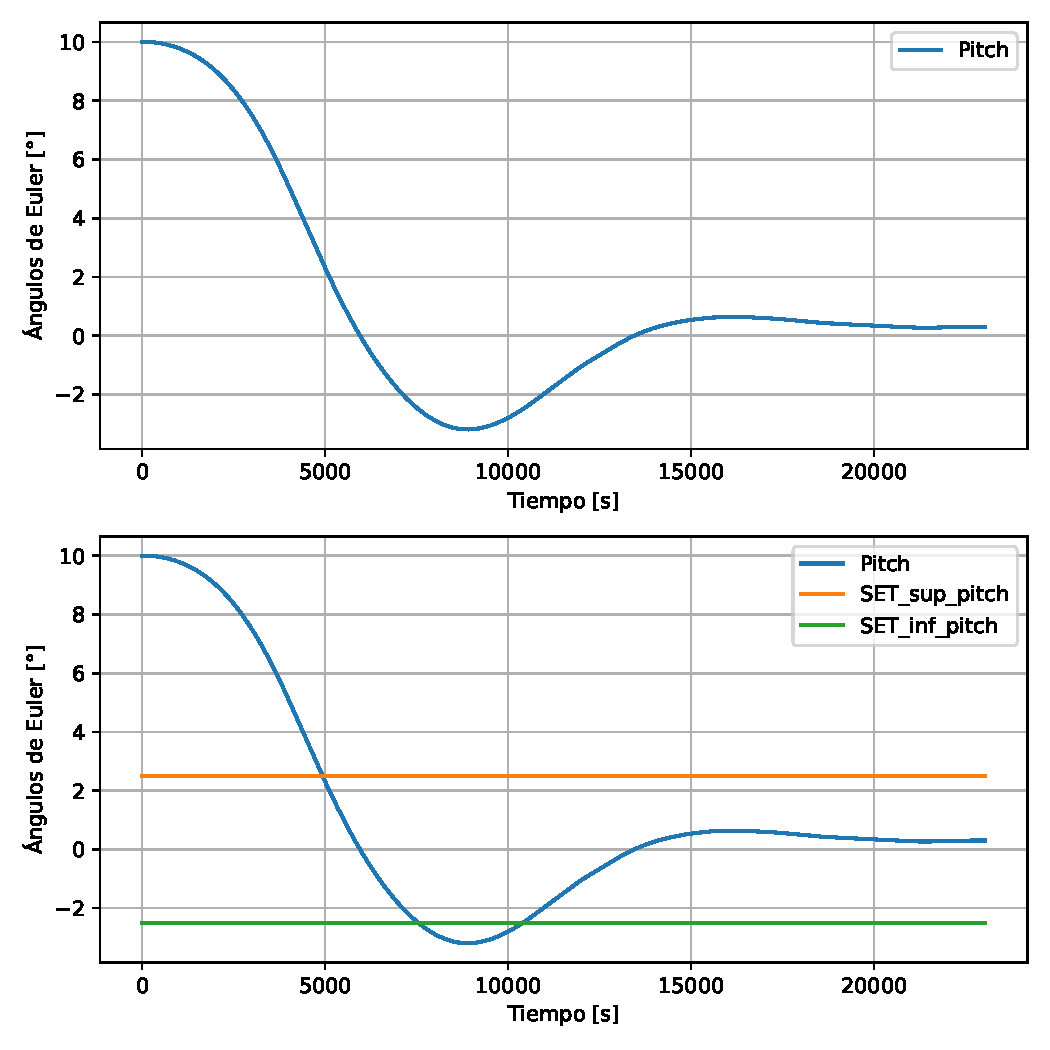
\includegraphics[width=0.6\textwidth]{time_pitch.pdf}
	\caption{Banda de asentamiento Pitch en modelo dinámico.}
	\label{fig:time_pitch}
\end{figure}	

\begin{figure}[H]
	\centering    
	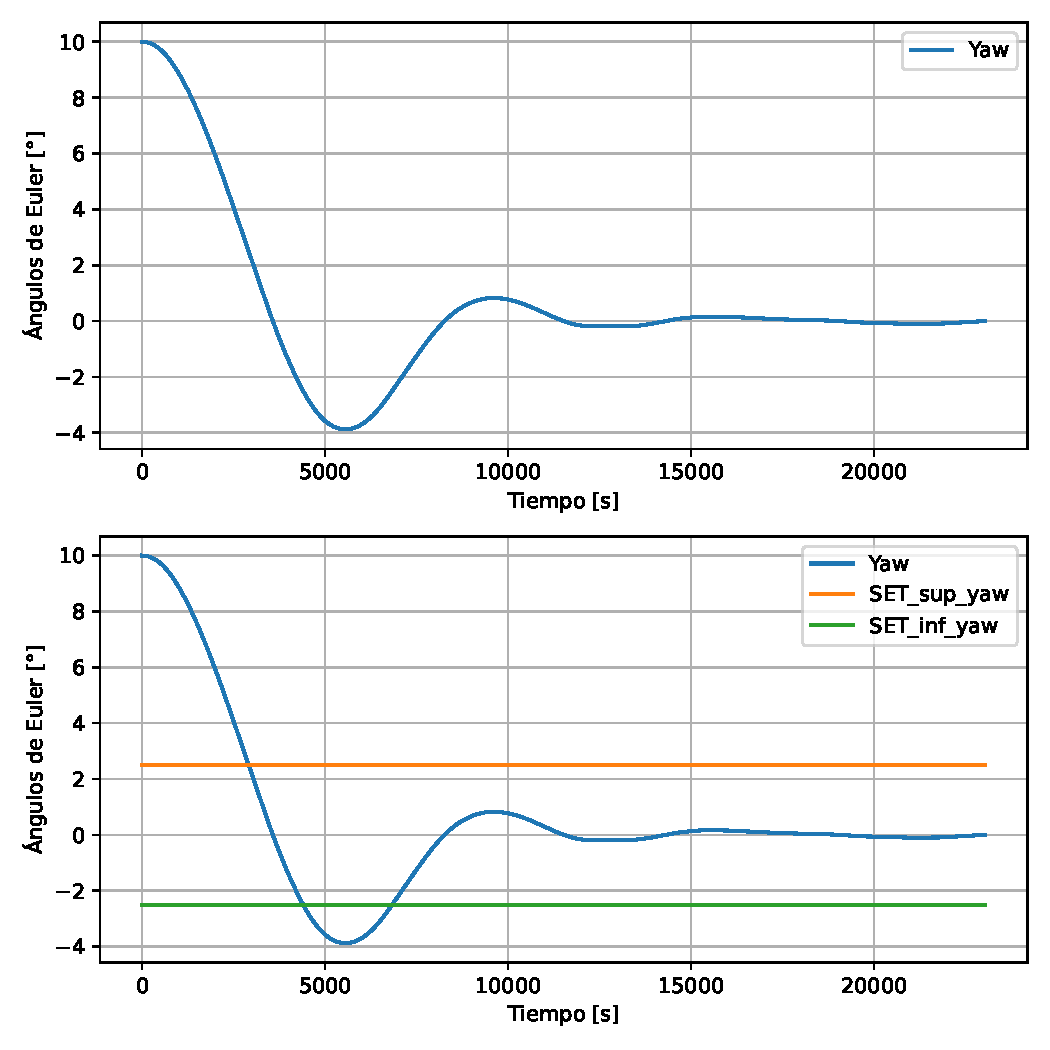
\includegraphics[width=0.6\textwidth]{time_yaw.pdf}
	\caption{Banda de asentamiento Yaw en modelo dinámico.}
	\label{fig:time_yaw}
\end{figure}	

\underline{Exactitud de apuntamiento}

ara evaluar la exactitud de apuntamiento en sus tres componentes, se utilizan los valores de los ángulos de Euler estimados, obtenidos tras el tiempo de asentamiento. A continuación, se calcula la desviación estándar de los valores que se encuentran dentro de la banda de asentamiento, es decir, aquellos que se acercan cada vez más al equilibrio, con dispersiones provocadas por el ruido y mitigadas mediante el uso de un filtro de Kalman. La exactitud de apuntamiento se expresa como tres veces la desviación estándar calculada en dicho periodo de tiempo, lo que representa que el 99.73\% de las orientaciones del satélite estarán dentro de este intervalo de confianza. A continuación, en las Figuras \ref{fig:roll_DNormal}, \ref{fig:pitch_DNormal} y \ref{fig:yaw_DNormal}, se muestran los histogramas que representan la distribución normal obtenida en este caso de ejemplo.


\begin{figure}[H]
	\centering    
	\includegraphics[width=0.65\textwidth]{roll_DNormal.pdf}
	\caption{Histograma de valores con distribución normal en Roll.}
	\label{fig:roll_DNormal}
\end{figure}	

\begin{figure}[H]
	\centering    
	\includegraphics[width=0.65\textwidth]{pitch_DNormal.pdf}
	\caption{Histograma de valores con distribución normal en Pitch.}
	\label{fig:pitch_DNormal}
\end{figure}	

\begin{figure}[H]
	\centering    
	\includegraphics[width=0.65\textwidth]{yaw_DNormal.pdf}
	\caption{Histograma de valores con distribución normal en Yaw.}
	\label{fig:yaw_DNormal}
\end{figure}	
